\section*{Results}

\subsection{The information contained in a window}

A recurrent process carries its state forward,
$\rho_t=\Phi_{a_t}(\rho_{t-1})$, and produces the scalar output
$Y_t=\operatorname{Tr}(O\rho_t)$.  A reset-window learner receives only
$S_t^{(d)}=(a_{t-d+1},\ldots,a_t)$ and returns a function of that suffix.  It
may use any quantum or classical feature map and any stateless readout.

Let $D_d$ be the largest output difference between two admissible histories
that have the same last $d$ inputs.  Let $E_d$ be the smallest worst-case error
among all functions of that window.  Then
\begin{equation}
 \begin{split}
 D_d&=\sup_{S_d(h)=S_d(h')}|Y(h)-Y(h')|,\\
 E_d&=\inf_{g_d}\sup_h|Y(h)-g_d(S_d(h))|=\frac{D_d}{2}.
 \end{split}
 \label{eq:window-law}
\end{equation}
The proof is immediate.  Two histories with the same window must receive the
same prediction $a$.  If their correct outputs are $y$ and $y'$, then
$|y-y'|\leq|y-a|+|y'-a|$, so one error is at least half their gap.  Conversely,
for each window, predict the midpoint between the infimum and supremum of its
compatible outputs.  Its error is at most half that range.  Taking the
supremum over windows proves Eq.~\eqref{eq:window-law}; values approaching the
two endpoints give the lower bound when an endpoint is not attained.

Equation~\eqref{eq:window-law} is the complete information test.  If $D_d=0$,
that window is exact.  If $D_d\to0$, longer windows approximate the output to
arbitrary accuracy.  If
$D_d\geq\Delta>0$ for every $d$, every finite-window predictor has error at
least $\Delta/2$.  Randomization does not remove the obstruction because the
prediction distribution is still identical for identical windows.  The
criterion concerns the declared output: state information that never reaches
the measurement does not contribute.

\subsection{Fading memory can be replaced by a window}

Write $D_{\rm tr}(\rho,\sigma)=\tfrac12\|\rho-\sigma\|_1$.  For scalar inputs
$u,v\in[0,1]$, suppose the channels obey the uniform incremental bound
\begin{equation}
 \begin{split}
 D_{\rm tr}(\Phi_u(\rho),\Phi_v(\sigma))
   &\leq\eta D_{\rm tr}(\rho,\sigma)\\[-2pt]
   &\quad+L_u|u-v|,
   \qquad 0\leq\eta<1,\\
 D_d&\leq2M\eta^d,
 \qquad E_d\leq M\eta^d .
 \end{split}
 \label{eq:incremental-channel}
\end{equation}
Here $M=\|O\|_\infty$.  Setting $u=v$ shows that the state difference shrinks
once per common input, giving
$D_{\rm tr}(\rho_d,\rho_d')\leq\eta^d$, while a bounded observable turns trace
distance into an output difference of at most $2M\eta^d$.  Thus a QRC
with uniform fading memory needs a window that grows only logarithmically with
the requested inverse accuracy.

The same inequality makes the replay output Lipschitz-continuous in the retained
inputs.  Encode each of the $d$ coordinates into $r$ fresh qubits and group
computational-basis outcomes by their blockwise Hamming weights.  These
probabilities form the multivariate Bernstein basis
\cite{goto2021universal,yu2024nonasymptotic}.

\textit{Reset-window emulation.}
For integers $d,r,Q\geq1$ and $0<\alpha<1$, there is a gate-based reset QELM
with $n=rd$ qubits and $B=(r+1)^d$ grouped outcomes.  Its exact-expectation
output $Q_{d,r}$ obeys a uniform bound, and for every fixed history $h$ its
$Q$-shot estimate $\widehat Q_{d,r,Q}$ obeys the pointwise bound
\begin{equation}
 \begin{aligned}
 \epsilon_{\rm hist}&=2M\eta^d,\\
 \epsilon_{\rm rep}&=\frac{ML_u(1-\eta^d)}{(1-\eta)\sqrt r},\\
 \epsilon_{\rm shot}&=M\sqrt{\frac{2\log(2/\alpha)}{Q}},\\
 \epsilon_{\rm tot}&=\epsilon_{\rm hist}+\epsilon_{\rm rep}+\epsilon_{\rm shot},\\
 \sup_h|Y(h)-Q_{d,r}(h)|
 &\leq\epsilon_{\rm hist}+\epsilon_{\rm rep},\\
 \Pr\!\left[|Y(h)-\widehat Q_{d,r,Q}(h)|\leq\epsilon_{\rm tot}\right]
 &\geq1-\alpha .
 \end{aligned}
 \label{eq:qrc-qelm-bound}
\end{equation}
The construction has three steps.  Replay the last $d$ QRC channels from one
fixed state; contraction bounds the discarded prefix by the first term.
Bernstein approximation represents the resulting continuous function of the
window and gives the second term.  Averaging the bounded score over $Q$ circuit
shots gives the third term.  The triangle inequality combines them.
The minimax certificate $E_d\leq M\eta^d$ may use the best midpoint for every
window; replay from one fixed state is constructive but gives the looser
$2M\eta^d$ term.

Each term can be made arbitrarily small.  Consequently, every continuous
fading-memory scalar QRC filter on a compact input interval is uniformly
approximable by a growing reset-QELM family: first choose a long enough window,
then a rich enough finite-window feature map.  This is an existence result for
a scalable family.  It gives neither universality to a fixed QELM architecture
nor an efficient method for learning the exponentially large coefficient
table.

\begin{figure*}[t]
 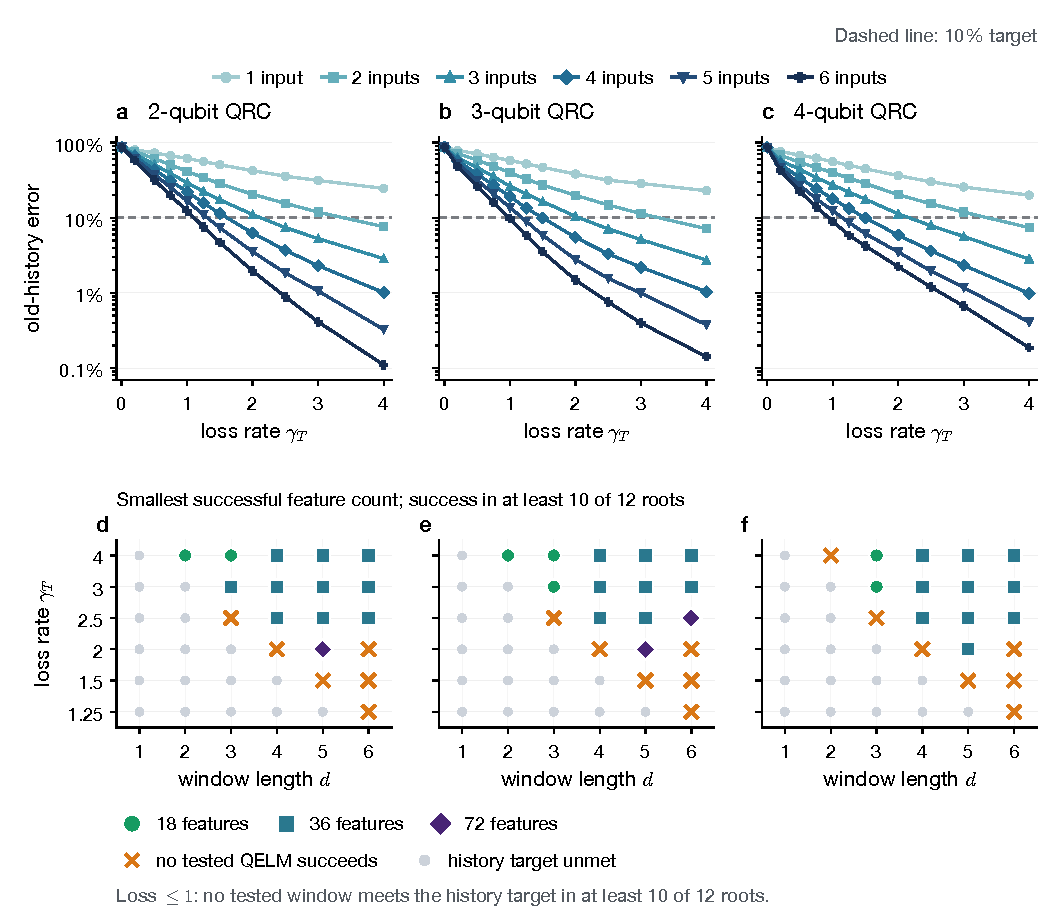
\includegraphics[width=\textwidth]{fig02_information_frontier.pdf}
 \caption{\textbf{When finite-window prediction becomes feasible.}
 For each displayed window, light gray means that output-relevant history
 remains outside that window at every tested feature budget.  Green, blue, and
 purple give the smallest successful budgets $B=18,36,72$, respectively, where
 success is the modal class across 12 independent roots at NRMSE tolerance
 $0.10$.  Orange is unresolved, and hatching marks root disagreement for at
 least one budget.  The map uses the frozen finite common-suffix panels drawn
 from the 33-symbol input alphabet.}
 \label{fig:information-frontier}
\end{figure*}

\subsection{Protected quantum memory cannot be replaced by a finite window}

A lasting obstruction needs one state quantity that an old input changes,
later inputs preserve, and the readout can observe.  A two-qubit singlet mode
has all three properties.  Its projector is visible through two-body Pauli
correlations, and symmetric channels leave it unchanged:
\begin{equation}
 \begin{aligned}
 P_-&=|\psi^-\rangle\!\langle\psi^-|
 =\frac{II-XX-YY-ZZ}{4},\\
 \Phi_{(u,0)}^\dagger(P_-)&=P_- .
 \end{aligned}
 \label{eq:protected-singlet}
\end{equation}
Here each time step uses the same time-homogeneous alphabet $a=(u,q)$.
The continuous value $u$ drives both qubits symmetrically; the flag $q$ applies
an addressable pulse to the first qubit.  After the old flagged input, the
allowed suffixes have arbitrary symmetric drives and $q=0$.  Exchange symmetry
and collective loss protect $P_-$, whereas the old local pulse changes its
population by
$\Delta p_-=\tfrac12\sin^2(0.5)=0.1149244235$.

Fix one infinite symmetric drive stream.  Two trajectories differ at the old
flagged input only and share every later input.  For a window of length $d$, we
evaluate after $d$ shared inputs.  The learner therefore sees identical data,
while the recurrent outputs retain the same gap.  For the two branches weighted
equally, let $R_{\rm pair}$ denote their mean squared prediction error.
Equation~\eqref{eq:window-law} and the appendix identity give
\begin{equation}
 \begin{aligned}
 E_d&\geq0.0574622 &&\text{for every finite }d,\\
 R_{\rm pair}&\geq0.0033019058 .
 \end{aligned}
 \label{eq:protected-floor}
\end{equation}
The same fixed recurrent process and fixed trajectory pair witness every
window.  The filter is therefore outside the fading-memory regime for the
declared output and symmetry-preserving suffix alphabet.

Numerical propagation over 12 independent couplings preserves the output gap
under collective loss to a maximum drift of $7.63\times10^{-16}$ through 80
suffix inputs.  Replacing collective by matched local loss reduces the median
gap to $1.57\times10^{-5}$ at step 80.  Small symmetry violations give a finite
certified persistence horizon; the short derivation is included below.

The information law itself is classical: any stateless window model faces the
same missing input.  The quantum physics lies in the mechanism that stores the
input, protects it with an open-system symmetry, and exposes it through Pauli
measurements.  Entanglement alone is not the obstruction.
